%! Author = jbf
%! Date = 31.07.25
\newpage
\section{Analyse und Konzeption}
\label{sec:analyse-und-konzeption}


In diesem Kapitel werden die grundlegenden Anforderungen und konzeptionellen
Überlegungen für die Entwicklung der Webapplikation beschrieben.
Ziel ist es, eine fundierte Basis für die spätere Implementierung zu schaffen, indem sowohl die
funktionalen als auch die nicht-funktionalen Anforderungen analysiert und geeignete technische Konzepte erarbeitet werden.
Dazu werden zunächst die Ausgangssituation und die zu verarbeitenden Datenquellen untersucht.
Die erarbeiteten Konzepte bilden die Grundlage für das Design und die Realisierung der Software im weiteren Verlauf der Arbeit.


\subsection{Definition der Anforderungen}
\label{sec:definition-der-anforderungen-und-ihre-interpretation}

In diesem Abschnitt werden die funktionalen und nicht-funktionalen Anforderungen der zu entwickelnden Web-Applikation beschrieben.
Sie wurden in Abstimmung mit den späteren Nutzerinnen und Nutzern sowie den betreuenden Personen im Unternehmen festgelegt.
Die Anforderungen bilden die Grundlage für den Entwurf und die Umsetzung der Software und dienen dazu, deren Zielsetzung, Funktionsumfang und technische Rahmenbedingungen klar zu definieren.


\subsubsection{Funktionale Anforderungen}\label{subsec:funktionale-anforderungen}

Die funktionalen Anforderungen beschreiben die vorgesehenen Funktionen und Abläufe der Applikation.
Sie definieren, was die Anwendung leisten soll und wie die Nutzerinnen und Nutzer mit ihr interagieren können.

\begin{enumerate}
  \item Navigation und Benutzerführung \\
  Die Applikation soll eine einfache und übersichtliche Navigation ermöglichen.
  Der Wechsel zwischen den Hauptfunktionen erfolgt über eine feststehende Menüleiste im oberen Bereich der Benutzeroberfläche.
  Dadurch können die Bereiche Upload, Berichte und Analyse direkt aufgerufen werden.

  \item Einlesen von XML-Dateien \\
  Das Einlesen der automatisch generierten XML-Berichte erfolgt über eine Upload-Seite.
  Die Anwendung soll sowohl ältere als auch neuere XML-Strukturen verarbeiten können, da der Teststand unterschiedliche Versionen erzeugt.

  \item Datenverarbeitung und Speicherung \\
  Nach dem Upload sollen die XML-Dateien automatisch geparst, validiert und in die Datenbank überführt werden.
  Doppelte Einträge sollen erkannt und vermieden werden.

  \item Anzeige der Berichte \\
  Die gespeicherten Berichte sollen tabellarisch dargestellt werden.
  Jede Zeile repräsentiert einen Testbericht und zeigt die wichtigsten Informationen wie Datum, Seriennummer, Materialnummer und Testergebnis an.

  \item Filter- und Suchfunktionen \\
  Die Berichtstabelle soll über Filteroptionen verfügen, um gezielt nach bestimmten Kriterien
  (z.\,B. Datum, Seriennummer, Testmodul oder Ergebnisstatus) zu suchen.

  \item Grafische Darstellung der Testdaten \\
  Die Anwendung soll die Messergebnisse der einzelnen Module grafisch darstellen.
  Die Diagramme sind nach Modulen sortiert und enthalten eine klare Achsenbeschriftung sowie Legenden.
  Das Layout der Diagramme soll sich an den Graphen des Teststandprogramms orientiert, um den Nutzerinnen und Nutzern die Interpretation zu erleichtern.

  \item Systemmeldungen und Fehlermanagement \\
  Nach erfolgreichen oder fehlerhaften Aktionen (z.\,B. Upload, Datenbankeintrag, Filterabfrage) sollen entsprechende Systemmeldungen angezeigt werden, um den Benutzerstatus transparent zu machen.

  \item Exportfunktionen \\
  Die Anwendung soll die Möglichkeit bieten, ausgewählte Graphen in ein externes Format zu exportieren.
  Dadurch können die Graphen auch außerhalb der Anwendung weiterverarbeitet werden.
\end{enumerate}

\subsubsection{Nicht-funktionale Anforderungen}
\label{subsec:nicht-funktionale-anforderungen}

Die nicht-funktionalen Anforderungen beschreiben die Qualitätsmerkmale der Software.
Sie legen fest, unter welchen Bedingungen die Applikation betrieben werden soll und welche Eigenschaften sie erfüllen muss.

\begin{enumerate}
  \item Plattform und Laufzeitumgebung \\
  Die Web-Applikation wird auf einem unternehmenseigenen Apache2-Server betrieben.
  Sie basiert auf Python und dem Webframework Flask.

  \item Performance \\
  Das System muss auch bei größeren XML-Dateien zuverlässig arbeiten.
  Hierbei wird von XML-Daten mit einer Vielzahl von Testmodulen ausgegangen.
  Eine aktive Laufzeitoptimierung ist nicht erforderlich, solange der Arbeitsfluss nicht beeinträchtigt wird.

  \item Usability \\
  Die Benutzeroberfläche soll intuitiv bedienbar sein und eine klare Struktur aufweisen.
  Eingabefehler sollen vermieden und, wenn möglich, automatisch erkannt werden.

  \item Modularität und Wartbarkeit \\
  Die Applikation ist modular aufgebaut, um eine einfache Pflege und spätere Erweiterung zu ermöglichen.
  Änderungen an einzelnen Komponenten sollen keine Anpassungen an anderen Modulen erfordern.

  \item Sicherheit und Datenintegrität \\
  XML-Dateien müssen vor dem Einlesen auf korrekte Struktur und mögliche Sicherheitsrisiken geprüft werden
  (z.\,B. Schutz vor fehlerhaften oder manipulierten Dateien).

  \item Fehler- und Ausnahmebehandlung \\
  Unerwartete Systemfehler sollen abgefangen und im Log gespeichert werden.
  Für Benutzerinnen und Benutzer werden stattdessen verständliche Fehlermeldungen ausgegeben.

  \item Skalierbarkeit \\
  Das System soll bei Bedarf mit minimalem Aufwand um zusätzliche Funktionen, Testmodule oder Datenquellen erweitert werden können.

  \item Kompatibilität \\
  Die Applikation soll auf allen gängigen Browsern lauffähig sein (z.\,B. Chrome, Edge, Firefox).

  \item Dokumentation und Nachvollziehbarkeit \\
  Der Code soll übersichtlich dokumentiert werden.
  Wichtige Abläufe (Upload, Datenverarbeitung, Visualisierung) werden nachvollziehbar beschrieben.
\end{enumerate}

\subsubsection{Anforderungen an die Datenbank}
\label{subsec:anforderungen-an-die-datenbank}

Die Datenbank ist ein zentraler Bestandteil der Anwendung.
Sie speichert alle relevanten Testdaten, Parameter und Informationen aus den XML-Berichten.

\begin{enumerate}

  \item Datenbanksystem \\
  Die Datenbank basiert auf dem relationalen Datenbanksystem MariaDB.

  \item Vollständige Abbildung der XML-Daten \\
  Sie muss in der Lage sein, sämtliche in den XML-Berichten enthaltenen Daten vollständig abzubilden,
  um die Wiederherstellung eines gesamten Testberichts theoretisch zu ermöglichen.

  \item Vermeidung von Datendopplungen \\
  Datendopplungen sollen vermieden werden.
  Häufig vorkommende Informationen (z.\,B. Teststandname, Versionsnummern, DUT-Typen) werden ausgelagert und über Fremdschlüssel referenziert.

  \item Strukturierung von Gerätedaten \\
  Für DUT-Typen und Seriennummern werden separate Informationstabellen angelegt,
  um Redundanzen zu vermeiden und die Datenstruktur klar zu halten.

  \item Erweiterbarkeit der Datenbankstruktur \\
  Die Datenbankstruktur soll so gestaltet sein, dass zukünftige Teststände oder zusätzliche Testmodule problemlos integriert werden können.

  \item Versionierung und Migration \\
  Änderungen an der Datenbankstruktur werden verwaltet,
  um eine konsistente Weiterentwicklung der Datenbank sicherzustellen.

  \item Datenvalidierung und Konsistenzprüfung \\
  Beim Einfügen neuer Datensätze sollen Validierungen sicherstellen,
  dass die Werte logisch und formal korrekt sind (z.\,B. keine Nullwerte bei Pflichtfeldern, korrekte Datentypen).
\end{enumerate}

Die beschriebenen Anforderungen bilden den Rahmen für die Entwicklung der Web-Applikation.
Während die funktionalen Anforderungen die konkreten Aufgaben und Abläufe definieren,
legen die nicht-funktionalen Anforderungen fest, wie die Anwendung qualitativ umgesetzt werden soll.
Zusammen mit den Datenbankanforderungen bilden sie die Grundlage für den folgenden Entwurf der Systemarchitektur und die spätere Implementierung.

\subsection{Grundlegender Ablauf des Programmes}
\label{subsec:grundlegender-ablauf-des-programmes}

\begin{figure}[H]
    \centering
    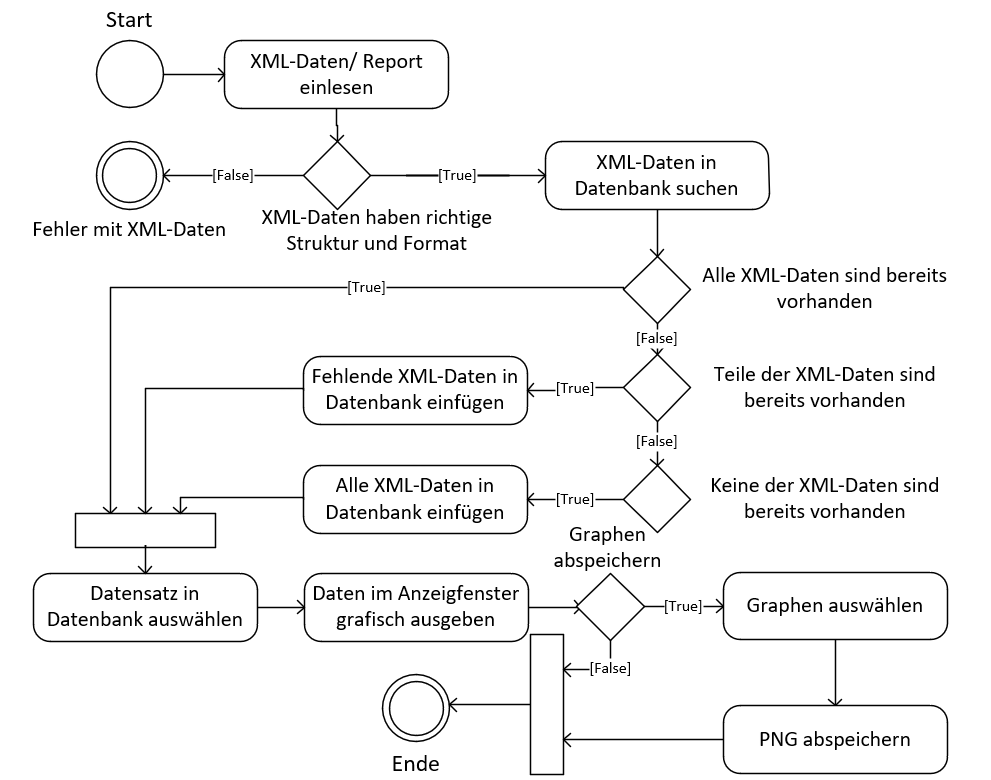
\includegraphics[width=0.95\textwidth]{Grafiken/Ablaufdiagramm}
    \caption{Grundlegedes Ablaufdiagramm der Nutzung der Web-Applikation}
    \label{fig: Grundlegedes Ablaufdiagramm der Nutzung der Web-Applikation}
    {Quelle: Eigene Darstellung mit Microsoft Visio}
\end{figure}
\subsection{Analyse der generierten XML-Berichte und bestehenden Strukturen}
\label{subsec:analyse-der-generierten-xml-berichte-und-bestehenden-strukturen}

In diesem Unterkapitel wird der Aufbau der automatisch
generierten Testberichte aus dem Teststand und der vorhandenen Ausgabe- und Speicherstruktur
erläutert. Dies ist relevant für die Erstellung der Datenbank und das
Verständnis der Ein- und Auslesefunktionen der Web-Applikation.

\subsubsection{XML-Berichtsstrukturschema}

Die vom Teststand automatisch generierten
Berichte folgen einem konstanten Strukturschema, welches sich bis zu einer
gewissen Ebene der XM-Struktur in jedem Bericht wiederholt. Wie im Kapitel „Grundlagen“
beschrieben, kann ein Element Attribute, andere Elemente und einen Inhaltswert beinhalten.

Das Stammelement heißt in allen automatisch
generierten Berichten „test“ und besitzt immer das Attribut „id“. Die Zahl in
diesem Attribut beschreibt den Typ des \ac{DUTs} die in diesem Test geprüft wurden.

Das Stammelement hat die Unter- bzw.
Kinderelemente „info“, „testbench“, „string“ und dreimal „testmodule“. Diese
Elemente haben wiederum alle weiter Unterelemente und Attribute.

Jedes der Elemente „testmodule“ hat ein Attribut
„name“, durch welches Sie unterschieden werden können. Das Element „string“ hat
ein Namensattribut mit der Bezeichnung „test sequence status“. Der Inhalt
dieses Elementes gibt an, ob der Test erfolgreich abgeschlossen wurde oder ob
es einen Fehler bzw. eine Grenzüberschreitung von Messwerten gab.
Die hier genannten eigenschaften sind in der Abbildung \ref{fig: Direkte Kinderelement unter Stammelement} zu erkennen.

\begin{figure}[H]
\centering
\begin{minipage}{0.95\textwidth}
\begin{lstlisting}[language=XML]
<?xml version="1.0" encoding="UTF-8"?>
    <test id="124">
    <info></info>
    <testbench></testbench>
    <testmodule name="DriverConsumptionTest"></testmodule>
    <testmodule name="PulseTest FSW L"></testmodule>
    <testmodule name="XPowerTest"></testmodule>
    <string name="test sequence status">
        Test sequence successfully finished.</string>
    </test>
\end{lstlisting}
\end{minipage}
\caption{Direkte Kinderelement unter Stammelement}
\label{fig: Direkte Kinderelement unter Stammelement}
    {Quelle: Eigene Darstellung}
\end{figure}


Das Element „info“ enthält in seinen Unterelementen die allgemeinen Testinformationen, wie die Startzeit des Tests,
die Typen-ID, die Konfigurationsbezeichnung des Teststandes, die Bezeichnung des angeschlossenen Carriers und die
Seriennummern des \ac{DUTs}. Diese Elemente haben keine Unterelemente und sind alle mit einem Namensattribut und einem Inhalt definiert.
Für die genauen Bezeichnungen und Struktur siehe Abbildung \ref{fig: XML-Strukturbeispiel Info-Element}

\begin{figure}[H]
\centering
\begin{minipage}{0.95\textwidth}
\begin{lstlisting}[language=XML]
<info>
	<string name="Time">2023-09-21_08:36:33</string>
	<string name="Material_number">124</string>
	<string name="Configuration">L_3DUT_3P1Q</string>
	<string name="ID_Carrier_left">Carrier 1</string>
	<string name="ID_DUT_R">10-29550</string>
	<string name="ID_DUT_S">10-29396</string>
    <string name="ID_DUT_T">10-29482</string>
</info>
\end{lstlisting}
\end{minipage}
\caption{XML-Strukturbeispiel Info-Element}
\label{fig: XML-Strukturbeispiel Info-Element}
    {Quelle: Eigene Darstellung}
\end{figure}

Die Teststandbezeichnung und die Versionen der Hard- und Software werden im Element „testbench“ gespeichert.
Diese Elemente enthalten auch keine weiteren Unterelemente und sind alle mit einem Namensattribut und einem Inhalt versehen.
Die genauen Bezeichnungen und die Struktur sind in Abbildung \ref{fig: XML-Strukturbeispiel Testbench-Element} zu sehen.

\begin{figure}[H]
\centering
\begin{minipage}{0.95\textwidth}
\begin{lstlisting}[language=XML]
<testbench>
	<string name="Testbench_name">USTB_DtWind</string>
	<string name="Testbench_HW_revision">V1.5</string>
	<string name="Version_GUI">V1.4.1</string>
    <string name="Version_controller">V1.3.2</string>
</testbench>
\end{lstlisting}
\end{minipage}
\caption{XML-Strukturbeispiel Testbench-Element}
\label{fig: XML-Strukturbeispiel Testbench-Element}
    {Quelle: Eigene Darstellung}
\end{figure}


Die Testmodule-Elemente sind alle nach dem gleichen Schema aufgebaut. Die ersten Unterelemente enthalten Grundinformationen
zu dem Status des Testmoduls, der Tages- und Uhrzeit des Tests und welche Versionen davon verwendet wurden.
Danach befinden sich noch drei weitere Elemente im Element „module“.
Diese Elemente heißen „Phase_U“, „Phase_V“ und „Phase_W“.
Sie besitzen kein Namensattribut.
Diese enthalten die Parameter und die Messdaten für die DUTs. Jede Phase enthält die Messwerte für ein DUT.
Somit besitzen alle Module unter dem Element „Phase_U“ die Messwerte und Parameter für den ersten DUT, dessen Seriennummer
unter dem Element mit dem Namensattribut „ID_DUT_R“ in Abbildung \ref{fig: XML-Strukturbeispiel Info-Element} zu finden ist.

In dem Element „parameters“, welches in jedem Phasenelement vorkommt, befinden sich die voreingestellten Rahmbedingungen
und Anforderungen für das Testmodul. Diese enthalten alle ein Namensattribut und einen Inhalt.

Die Elemente unter dem Eintrag „measurements“ enthalten die Messdaten der Testmodule. Sie haben oft noch extra Attribute
wie „min“ oder „max“, welche die Toleranzgrenzen beschreiben. Diese Toleranzgrenzen zeigen, in welchem Bereich der jeweilige
Elementinhalt angesiedelt sein muss, um kein positives bzw. fehlerfreies Ergebnis zu erzeugen.
Die meisten Attributswerte finden sich schon in den Parametern wieder und sind somit doppelt im Bericht zu finden.
Nur bei den Floatblock-Elementen, also Elementen mit der Bezeichnung Floatblock, sind besondere Attribute zu finden,
welche nicht gedoppelt vorkommen.
Diese Elemente umfassen zusätzlich die Attribute „size“ und „duration“, welche die Anzahl der in dem Inhalt enthaltenen
Floatwerte und die Dauer der Werteaufnahme angeben.
Diese sind für die grafische Darstellung besonders relevant.

Dies auf der Phasenebene: Treten keine Veränderungen in der XML-Struktur auf, variieren lediglich die Elemente unter den
Phasenelementen von Bericht zu Bericht etwas.
Die beträchtliche Ausnahme von dieser Regel bilden die Berichte, bei denen ein Fehler aufgetreten ist oder sogar der
Testvorgang abgebrochen wurde. Bei diesen Berichten hört die XML-Struktur bei den fehlgeschlagenen Testmodulen schon auf.
Der Testbericht ist aber in sich geschlossen. Das bedeutet, die XML-Struktur ist vollkommen und kann von einem XML-Parser eingelesen werden.
Es befinden sich nur weniger Testmodul-Elemente in dem Bericht und im Element für den Testsequenzstatus ist folgender Inhalt
enthalten: „Test sequence finished with errors.“ Zudem wird bei dem Testmodul, bei dem der Fehler aufgetreten ist, unter
dem Element mit dem Namen „Testresult“ ein Fehlercode und seine Bedeutung ausgegeben. In Abbildung \ref{} ist ein
Beispiel für einen Bericht, welcher beim ersten Testmodul einen Fehler ausgegeben hatte.
Bei einem Ausfall eines der zu testenden DUTs gibt es die Besonderheit, dass die anderen noch funktionsfähigen DUTs
keine weiteren Datenaufnahmen mehr machen können. Denn das System benötigt alle drei Phasen, um den Test durchzuführen.
Die XML-Struktur ist in sich geschlossen, aber es werden keine Daten von den anderen DUTs mehr aufgenommen.








\subsection{Datenbankdesign und Strukturkonzeption}
\label{subsec:datenbankdesign-und-strukturkonzeption}
\input{Kapitel/2. Hauptteil/3. Analyse und Konzeption/3.4 Grundkonzept des Benutzeroberflächen-Design}
\subsection{Entwurf der Applikationsarchitektur}
\label{subsec:entwurf-der-applikationsarchitektur}


Der Entwurf der Applikationsarchitektur bildet die konzeptionelle Grundlage für die technische Umsetzung der entwickelten Web-Applikation.
Das Ziel ist es, eine Struktur zu schaffen, die modular, wartbar und erweiterbar ist, und die gleichzeitig den funktionalen Anforderungen gerecht wird und sich in die bestehende Systemlandschaft integrieren lässt.
Die Architektur der Anwendung ist schichten- und komponentenorientiert aufgebaut und nutzt das Webframework Flask, welches eine klare Trennung zwischen der Präsentations-, Logik- und Datenhaltungsschicht ermöglicht.


\subsubsection{Architekturübersicht}

Die Applikation soll als serverbasierte Webanwendung im Client-Server-Modell funktionieren.
Das bedeutet: Während der Server die Datenverarbeitung, -speicherung und -bereitstellung übernimmt, ermöglicht der Client über den Webbrowser die Darstellung und Interaktion.
Die Anwendung ist in mehrere Schichten gegliedert, zu denen man die einzelnen Programmteile zuordnen kann.
Die Anwendung wird in folgende Schichten gegliedert:

\begin{itemize}
\item Präsentationsschicht (Frontend): Bereitstellung der Benutzeroberfläche über HTML-Templates, CSS und JavaScript.

\item
Applikationslogik (Backend): Implementierung der Geschäftslogik, Steuerung des Datenflusses und Verarbeitung der XML-Dateien.

\item
Datenhaltungsschicht: Persistente Speicherung der extrahierten Mess- und Gerätedaten in einer relationalen Datenbank mittels ORM.

\end{itemize}

Ein schematisches Architekturdiagramm dieser Struktur ist in Abbildung \ref{fig:arch_minimal} dargestellt.

\begin{figure}[H]
    \centering
    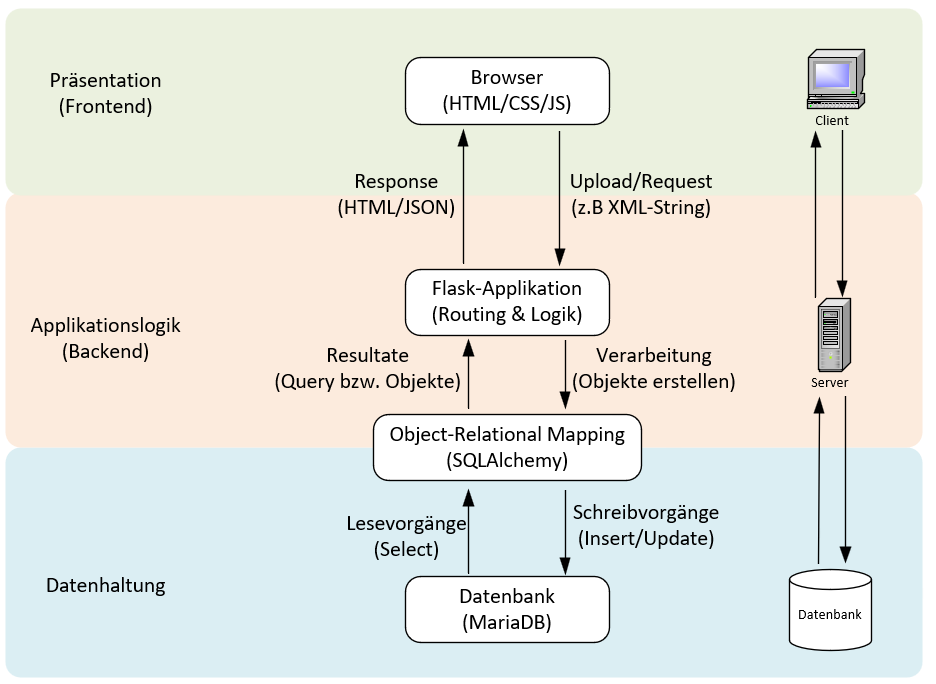
\includegraphics[width=0.95\textwidth]{Grafiken/Architekturdiagramm}
    \caption{schematisches Architekturdiagramm der Applikation}
    \label{fig:arch_minimal}
    {Quelle: Eigene Darstellung mit Microsoft Visio}
\end{figure}

\subsubsection*{Präsentationsschicht}

\begin{figure}[H]
  \centering
    \begin{minipage}{0.8\textwidth}
    \small
    Die Abbildung zeigt den Aufbau der Flask-Applikation.
    Im Verzeichnis \texttt{blueprints} befinden sich die einzelnen Routen-Module,
    während im Ordner \texttt{models} die Datenbankmodelle definiert sind.
  \end{minipage}
  \begin{minipage}{0.2\textwidth}
    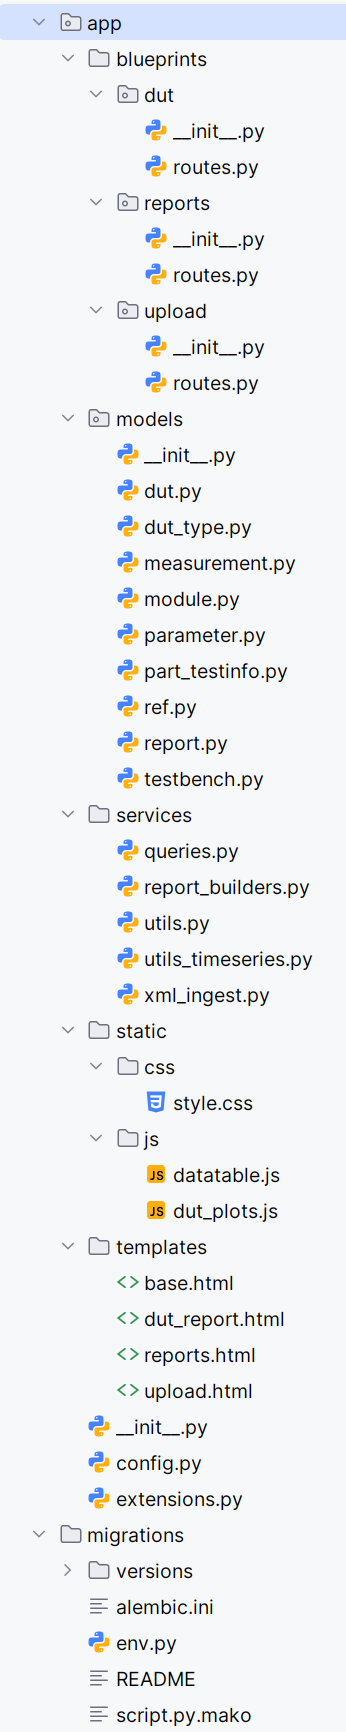
\includegraphics[width=0.9\textwidth, height=0.8\textheight, keepaspectratio]{Grafiken/App-Ordnerstruktur.png}
    \caption{Verzeichnisstruktur der Flask-Applikation}
    \label{fig:app-structure}
  \end{minipage}\hfill

\end{figure}

Die Präsentationsschicht besteht aus einer Kombination aus HTML-Templates und statischen Ressourcen (CSS, JavaScript), die im Verzeichnis templates/ bzw. static/ abgelegt sind.


\begin{itemize}

\item
Die Templates upload.html, reports.html und dut\_report.html bilden die Kernseiten der Weboberfläche.

\item
Statische Dateien wie style.css und dut\_plots.js dienen der Gestaltung und der interaktiven Darstellung von Messergebnissen.

Die Kommunikation mit der Logikschicht erfolgt über die definierten \textit{Flask Blueprints}, die als modulare Controller agieren.

\end{itemize}

\subsubsection*{Applikationslogik}

Die zentrale Geschäftslogik ist in modularen \textit{Blueprints} und \textit{Service-Komponenten} realisiert.

Die drei Blueprints upload, reports und dut kapseln die jeweiligen Funktionsbereiche:

\begin{itemize}

\item
upload: Einlesen und Validieren von XML-Dateien.

\item
dut: Verarbeitung und Anzeige der Daten eines „Device Under Test“.

\item
reports: Zusammenstellung und Ausgabe von Auswertungen.

\end{itemize}

Unterstützt werden diese durch das Modul services/, das die eigentliche Logik zur Datenverarbeitung bereitstellt:

\begin{itemize}

\item
xml\_ingest.py übernimmt das Parsen und Einlesen der XML-Daten.

\item
queries.py enthält vordefinierte Datenbankabfragen.

\item
utils.py und utils\_timeseries.py stellen Hilfsfunktionen zur Verfügung, z. B. zur Zeitreihenanalyse und Datenaufbereitung.

\item
report\_builders.py dient der Erstellung und Formatierung von Report-Daten für die grafische Darstellung.

\end{itemize}

Die Applikationslogik wird über die Datei run.py initialisiert, welche den Flask-Server startet und die Anwendungskonfiguration aus config.py einliest.


\subsubsection*{Datenhaltungsschicht}

Die Datenhaltung erfolgt über ein relationales Datenbanksystem, das über das Flask-eigene \textit{SQLAlchemy ORM} angebunden ist.

Die Datenmodelle sind im Verzeichnis models/ definiert und bilden die logischen Entitäten der Prüfanlage ab, darunter:

\begin{itemize}

\item
dut.py (Device Under Test)

\item
measurement.py (Messdaten)

\item
parameter.py (Prüfparameter)

\item
testbench.py, module.py und ref.py (Referenzdaten und Prüfaufbau)

\end{itemize}

Die Beziehungen zwischen den Modellen ermöglichen eine strukturierte und relationale Abbildung der Prüfdaten, wodurch eine effiziente Abfrage und Analyse möglich ist.

Migrationen werden mit \textit{Alembic} verwaltet, wie das Verzeichnis migrations/ zeigt.



\subsubsection{Kommunikation und Datenfluss}

Alles startet mit dem Hochladen einer XML-Datei über die Weboberfläche.
Der Blueprint upload übergibt die Datei an das Modul xml\_ingest, welches die XML-Struktur analysiert, relevante Informationen extrahiert und sie über die Datenmodelle in der Datenbank speichert.
 Die über den Blueprint reports oder dut gespeicherten Daten können anschließend abgerufen und visuell über die Templates dargestellt werden.
 Die Schichten kommunizieren ausschließlich über klar definierte Schnittstellen und ORM-Modelle, was eine lose Kopplung und eine hohe Wartbarkeit ermöglicht.









